\section{Anwendungsarchitektur}
\label{app_architecture}
Dieser Abschnitt beschreibt das implementierte System in der Gesamtheit. Es werden alle Komponenten client- und serverseitig vorgestellt. Die darauffolgenden Abschnitte widmen sich bestimmten Kernkomponenten detailliert. 

Das zu implementierende Werkzeug kann in zwei Bereiche gegliedert werden, dem Android-Client und dem HTTP-Server. Der Server

\subsection{Client-Server-Kommunikation}

\begin{figure}[h]
	\label{fig:architecture}
	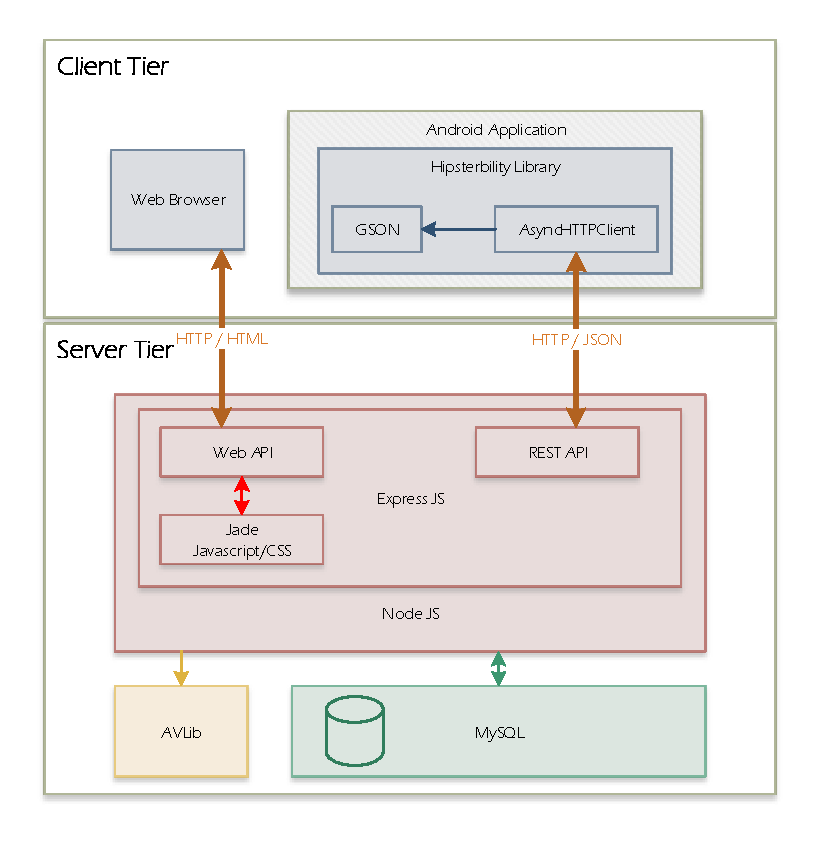
\includegraphics[width=\linewidth]{img/architecture}
	\caption{Hipsterbility Architektur}
\end{figure}
%TODO: write description, system requirements, Architekturbild ...

